       
%#####################################################################################################################			
%\subsection{Transport properties}
%\label{sec_TP}
%############################################################################################################################
\subsection {Viscosity} \label{sec-viscosity}
Many authors developed correlation equations for viscosity $\eta$ of fluids at a density $\rho$ and a temperature $T$. Those correlation equations may be composed of two or three terms, like

\begin{equation}
\eta (\rho,T) = \eta_{0} (T) + \eta_{ex} (\rho,T)
	\label{eq-two-term-visc}
\end{equation}

or

\begin{equation}
\eta (\rho,T) = \eta_{0} (T) + \Delta \eta (\rho,T) + \Delta \eta_c (\rho,T).
	\label{eq-three-term-visc}
\end{equation}


In the two-term form, the viscosity correlation consists of a zero-density limit viscosity $\eta_0(T)$ at a temperature $T$, and an excess contribution viscosity $\eta_{ex}(\rho,T)$ at a density $\rho$ and a temperature $T$. This type of correlation function is used (among others) by \textsc{Friend} et al.\ \cite{FriElyIng:89} or \textsc{Stephan} et al.\ \cite{SteKraLae:87}. The formulation can be enhaced by a term describing the viscosity in the immediate vicinity of the critical point, $\Delta \eta (\rho,T)$ \eqref{eq-three-term-visc}, as described in \textsc{Fenghour} et al.\ \cite{FenWakVes:98} or \textsc{Huber} et al.\ \cite{IAPWS:08a}. An overview about the used viscosity correlations for several substances is given in Tab.~\ref{tab-eos-visc}. To show an example, Fig.~\ref{fig-eos-visc-co2} portrays the resulting viscosities for carbon dioxide based on densities of different EOS.


\begin{table}[H]
  \caption{\label{tab-eos-visc}Ranges of $T$ and $p$ validity for viscosity correlations for several substances.}
  \begin{center}
  \begin{tabular}{lrrl}
  \toprule
  substance 		& $T$ [K]		& $p$ [MPa] 	& reference \\
  \midrule
  Carbon dioxide 	& 200--1500		& $\leq{300}$ 	& \cite{FenWakVes:98}\\
  Nitrogen       	& 70--1100		& $\leq{100}$ 	& \cite{SteKraLae:87}\\  
  Ethane         	& 90--625		& $\leq{30}$ 	& \cite{FriIngEly:91}\\ 
  Methane       	&	91--600		& $\leq{100}$	& \cite{FriElyIng:89}\\  
  Water          	& 273--1173		& $\leq{100}$	& \cite{IAPWS:08a}\\
  \bottomrule
 \end{tabular}
 \end{center}
\end{table}
  


%############################################################################################################################
\subsection {Thermal conductivity} \label{sec-thermal-conductivity}
%$~~$ \\
Similar to the correlations between viscosity and $T$ and $p$, the thermal conductivity $\lambda$ can be expressed by an equation consisting of the following three parts (see \cite{VesWak:90}): A conductivity in the limit of zero-density $\lambda^0(0,T)$, where only two-body interaction occurs, a term $\Delta_c\lambda (\rho,T)$ wich enhances the property function in the critical region of the fluid, and finally $\Delta\lambda (\rho,T)$ which represents the contribution of all other effects to the thermal conductivity at elevated densities including many-body collisions, molecular-velocity correlations and collisional transfer. This equation is

\begin{equation}
\lambda (\rho,T) = \lambda^0 (T) + \Delta\lambda (\rho)+ \Delta_c \lambda (\rho,T).
\label{EqEOS_visc}
\end{equation}

Fig.~\ref{fig-eos-hc-co2} shows the thermal conductivity of carbon dioxide at four temperatures based on different EOS. In Tab.~\ref{tab-eos-hc} the ranges for the validity of $T$ and $p$ concerning thermal conductivity correlations for several substances are shown.

\begin{table}[H]
 \caption{\label{tab-eos-hc}Ranges of $T$ and $p$ validity for thermal conductivity correlations for several substances.}
 \begin{center}
  \begin{tabular}{lrrl}
 \toprule
   substance 		& $T$ [K] 		& $p$ [MPa] 			& Reference \\
  \midrule
  Carbon dioxide 	& 200--1000		& $\leq{100}$ 			& \cite{FenWakVes:98}\\
  Nitrogen       	& 70--1100		& $\leq{100}$		 	& \cite{SteKraLae:87}\\  
  Ethane         	& $\leq{600}$	& $\leq{70}$		 	& \cite{YouEly:87}\\ 
  Methane       	& $\leq{200}$ 	& $\leq{600}$		 	& \cite{YouEly:87}\\  
  Water          	& $\leq{800}$ 	& $\leq{100}$		 	& \cite{IAPWS:08b}\\
  \bottomrule
 \end{tabular}
 \end{center}
\end{table}

%\begin{figure}
%\begin{minipage}{0.49\textwidth}
%\centering
%\includegraphics[width=1\textwidth]{FLUID_PROPERTIES/figures/viscosity-co2.eps}
%\caption[bild1]{Viscosity of $\mathrm{CO_2}$ based on different EOS}
%\label{fig-eos-visc-co2}
%\end{minipage}
%%
%\hspace{0.02\textwidth
%}
%\begin{minipage}{0.49\textwidth}
%\centering
%\includegraphics[width=1\textwidth]{FLUID_PROPERTIES/figures/heat-conductivity-co2.eps}
%\caption[bild2]{Thermal conductivity of $\mathrm{CO_2}$ based on different EOS}
%\label{fig-eos-hc-co2}
%\end{minipage}
%\end{figure}



\begin{figure}[t]
\subfigure[]{\label{fig-eos-visc-co2}\includegraphics[width=0.5\textwidth]{FLUID_PROPERTIES/figures/viscosity-co2.eps}}
\hfill
\subfigure[]{\label{fig-eos-hc-co2}\includegraphics[width=0.5\textwidth]{FLUID_PROPERTIES/figures/heat-conductivity-co2.eps}}
\caption[]{\label{fig-eos-visc-hc-co2}Viscosity~\subref{fig-eos-visc-co2} and thermal conductivity~\subref{fig-eos-hc-co2} of $\mathrm{CO_2}$ based on different EOS. There stand 
\setlength{\unitlength}{1ex}
\begin{picture}(5,1)
\thicklines \put(0,0.5){\line(1,0){5}}
\end{picture}
for the \textsc{Helmholtz} Free Energy,
\begin{picture}(5,1)
\thicklines \multiput(0,0.5)(2,0){3}{\line(1,0){1}}
\end{picture}
for the PREOS and
\begin{picture}(5,1)
\thicklines \multiput(0,0.5)(2,0){3}{\line(1,0){1}}\multiput(1.4,0.5)(2,0){2}{\line(1,0){0.25}}
\end{picture}
for the RKEOS. The colours refer to different temperatures (\textcolor{blue}{blue} - $\unit[280]{K}$, \textcolor{violet}{violet} - $\unit[320]{K}$, \textcolor{purple}{pink} - $\unit[400]{K}$, \textcolor{red}{red} - $\unit[680]{K}$).}
\end{figure}

